\documentclass[11pt,a4paper]{article}

\usepackage[margin=2.2cm]{geometry}
\usepackage{amsmath}
\usepackage{amssymb}
\usepackage{array}
\usepackage{booktabs}
\usepackage{longtable}
\usepackage{tikz}
\usetikzlibrary{arrows.meta,positioning,calc,shapes.multipart,shapes.geometric}
\usepackage{enumitem}
\usepackage{fancyhdr}
\usepackage{xcolor}
\usepackage{hyperref}
\usepackage{listings}
\usepackage{parskip}

\definecolor{boxblue}{RGB}{224,236,249}
\definecolor{boxgrey}{RGB}{237,237,237}
\definecolor{codebg}{RGB}{245,245,245}

\lstset{
  basicstyle=\ttfamily\small,
  backgroundcolor=\color{codebg},
  frame=single,
  framerule=0.3pt,
  columns=fullflexible,
  breaklines=true,
  xleftmargin=4pt, xrightmargin=4pt,
}

\setlength{\headheight}{14pt}
\pagestyle{fancy}
\fancyhf{}
\lhead{Computer Organization Lab}
\rhead{4-bit Accumulator CPU in Logisim-Evolution}
\cfoot{\thepage}

\newcommand{\task}[1]{\par\vspace{4pt}\noindent\textbf{Task #1}}
\newcommand{\checkoff}{\raisebox{-0.1em}{$\square$}\ }

\title{\textbf{Lab Sheet: Designing and Implementing a Simple\\ General-Purpose Microprocessor}\\[4pt]
\large A 4-bit Accumulator-Based CPU in Logisim-Evolution}
\author{Computer Organization / Digital Systems Laboratory}
\date{}

\begin{document}
\maketitle
\thispagestyle{fancy}

\section{Overview}

In this lab you will design and build a complete, working \textbf{general-purpose CPU}
inside Logisim-Evolution, starting from a provided Arithmetic Logic Unit (ALU) module
(\texttt{alu.circ}) and adding the remaining components required to make a
programmable machine: a \textbf{Program Counter (PC)}, an \textbf{Instruction
Register (IR)}, an \textbf{Accumulator (ACC)}, a \textbf{RAM/ROM} program
memory, and a small amount of \textbf{hardwired control logic}.

This machine deliberately uses the simplest possible organisation: \textbf{the
PC is the only address ever presented to memory} (there is no separate
address register, and no shared bus -- every connection is a direct,
point-to-point wire), and \textbf{there is no fetch/decode/execute state
machine to design}. Instead, every instruction's opcode bits, sitting right
there in the instruction word coming out of RAM, are wired straight into the
handful of gates that generate the load-enable and ALU-select signals. The
whole CPU updates its registers once per clock edge -- it is a
\emph{single-cycle} machine.

The instruction set is deliberately small (\textbf{9 instructions, including
one conditional and one unconditional branch}) so that the whole machine
stays small enough to design, debug, and fully understand within the lab
session.

\subsection*{Learning Outcomes}
By the end of this lab you will be able to:
\begin{itemize}[nosep]
  \item Explain how a CPU's datapath (registers, ALU, point-to-point wiring)
        executes an instruction in a single clock cycle.
  \item Derive simple combinational (\emph{hardwired}) control equations
        directly from an opcode encoding, without building a state machine.
  \item Wire registers, memory and an ALU together in Logisim-Evolution.
  \item Encode a small instruction set architecture (ISA) into binary opcodes,
        choosing the encoding so control logic stays simple.
  \item Hand-assemble and run simple machine-code programs (including loops
        and conditional branches) on your own CPU.
\end{itemize}

\section{Provided Component: The ALU (\texttt{alu.circ})}

You are given a working 4-bit ALU circuit, \texttt{ALU\_4}, with the following
interface:

\begin{center}
\begin{tabular}{@{}lcl@{}}
\toprule
\textbf{Pin} & \textbf{Width} & \textbf{Description} \\
\midrule
$A$ & 4 bits & First operand (input) \\
$B$ & 4 bits & Second operand (input) \\
$S$ & 3 bits & Function-select (input) \\
$F$ & 4 bits & Result (output) \\
\bottomrule
\end{tabular}
\end{center}

Internally, $A$ and $B$ feed an \textbf{Adder}, a \textbf{Subtractor}, a 4-bit
\textbf{AND} gate and a 4-bit \textbf{OR} gate in parallel; an 8:1
\textbf{Multiplexer} controlled by $S$ selects which result reaches $F$. Only
four of the eight possible select codes are wired up, giving the following
function table:

\begin{center}
\begin{tabular}{@{}ccl@{}}
\toprule
$S_2 S_1 S_0$ & Operation & $F$ \\
\midrule
\texttt{000} & ADD & $A + B$ \\
\texttt{001} & SUB & $A - B$ \\
\texttt{010} & AND & $A \wedge B$ \\
\texttt{011} & OR  & $A \vee B$ \\
\texttt{100--111} & --- & unused / reserved \\
\bottomrule
\end{tabular}
\end{center}

\task{1 --- Familiarisation.} Open \texttt{alu.circ} in Logisim-Evolution.
Test each of the four functions with a few input combinations using the
Poke tool, and confirm the function table above by observation. Keep a note
of the $S$ codes: you will wire $S$ directly from opcode bits later (\S 3).

\section{CPU Architecture}

You will build a small \textbf{single-accumulator CPU} with 4-bit data
width (matching the ALU) and a program/data memory of \textbf{16
locations $\times$ 8 bits} (4-bit address, 8-bit word). Following the
style of a classic hardwired-control datapath (Figure~\ref{fig:datapath}):

\begin{itemize}[nosep]
  \item \textbf{No shared bus.} Every connection is a dedicated
        point-to-point wire (or, where more than one value can reach the
        same place, a small 2:1 multiplexer) -- never a multi-driver line
        that needs arbitration.
  \item \textbf{No MAR.} RAM's address input is fed by a single 2:1 mux
        choosing directly between \texttt{PC} (fetching an instruction)
        and \texttt{IR[3:0]} (addressing the operand of the instruction
        just fetched). A multiplexer is combinational -- it is not a
        register, so there is still no separate ``address register''
        anywhere in the machine.
  \item \textbf{No fetch/decode/execute state machine.} All of the
        load-enable and select signals (\texttt{IRload}, \texttt{PCload},
        \texttt{MemWr}, \texttt{ACCload}, \dots) are generated by a small
        block of \emph{combinational} logic that reads the opcode bits
        sitting in \texttt{IR} directly -- this is called \textbf{hardwired
        control}, as opposed to a microprogrammed sequencer with states.
        The only sequential element besides the datapath's own registers
        is a single 1-bit \emph{Fetch/Execute phase} flip-flop, $T$
        (Figure~\ref{fig:phase}) -- not a multi-state FSM.
\end{itemize}

\begin{figure}[h!]
\centering
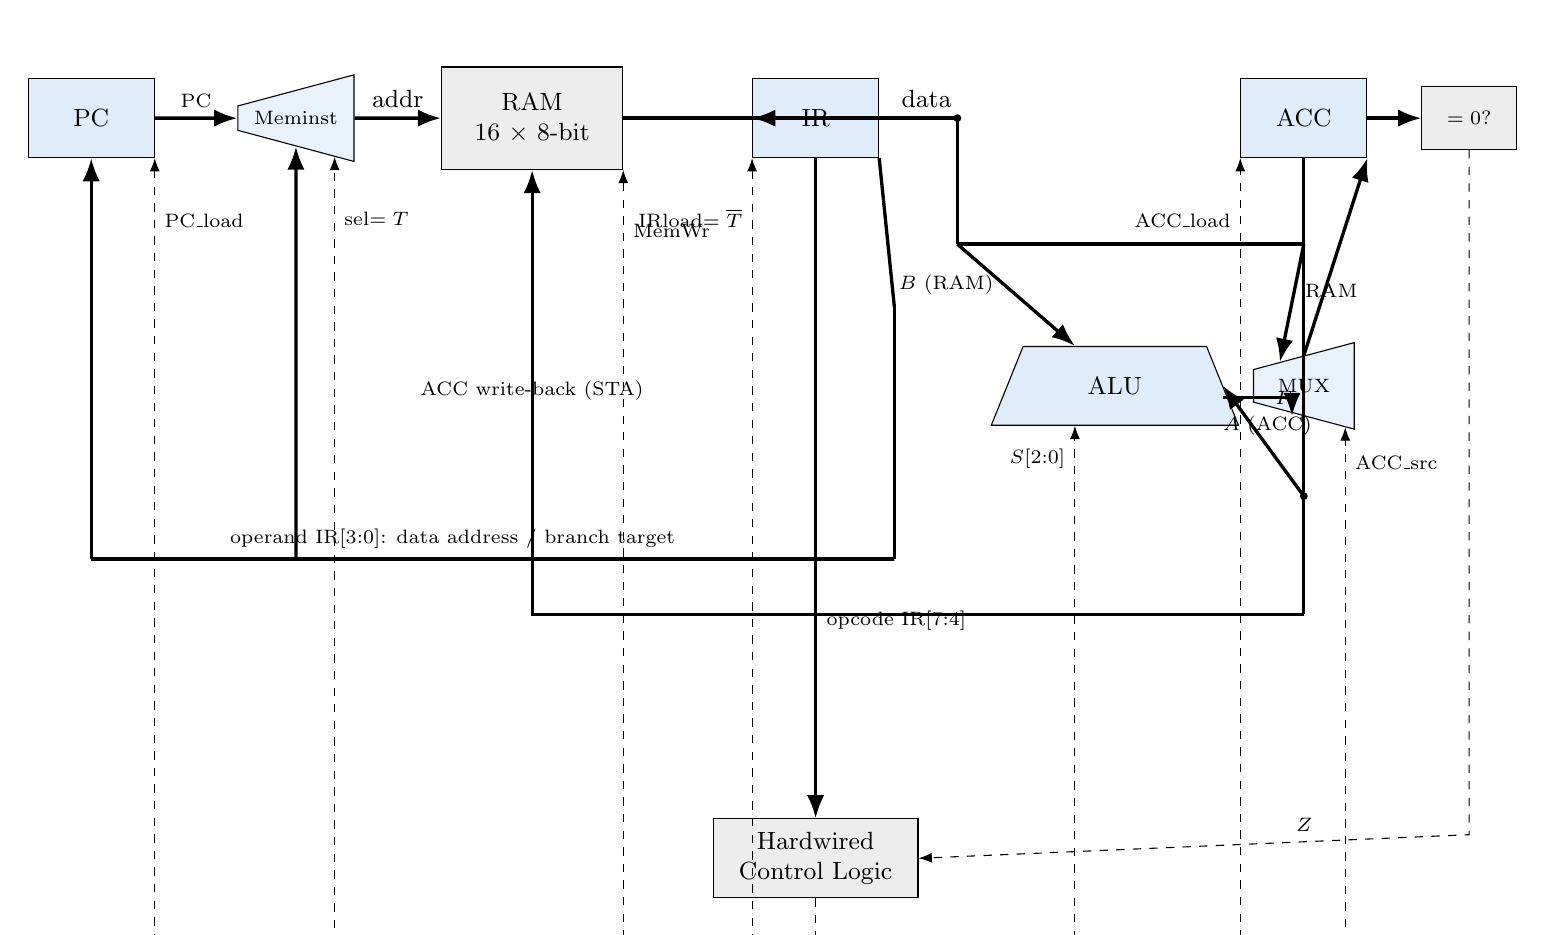
\begin{tikzpicture}[
  reg/.style={draw, fill=boxblue, minimum width=1.6cm, minimum height=1cm, font=\small, align=center},
  mem/.style={draw, fill=boxgrey, minimum width=2.3cm, minimum height=1.3cm, font=\small, align=center},
  ctl/.style={draw, fill=boxgrey, minimum width=2.6cm, minimum height=1cm, font=\small, align=center},
  small/.style={draw, fill=boxgrey, minimum width=1.2cm, minimum height=0.8cm, font=\scriptsize, align=center},
  alu/.style={draw, fill=boxblue, trapezium, trapezium angle=68, shape border rotate=-90,
              minimum width=1.5cm, minimum height=1cm, font=\small, align=center, inner sep=2pt},
  mux/.style={draw, fill=boxblue!70, trapezium, trapezium angle=75, shape border rotate=90,
              minimum width=1.1cm, minimum height=0.8cm, font=\scriptsize, align=center, inner sep=1pt},
  wire/.style={very thick},
  ctlsig/.style={-{Latex}, dashed},
  dot/.style={circle, fill, inner sep=1pt},
  every node/.style={font=\small}
]

% ---- main left-to-right dataflow row (y=7) ----
\node[reg] (pc)   at (0,7)     {PC};
\node[mux] (mmux) at (2.6,7)   {Meminst};
\node[mem] (ram)  at (5.6,7)   {RAM\\16 $\times$ 8-bit};
\node[reg] (ir)   at (9.2,7)   {IR};
\node[reg] (acc)  at (15.4,7)  {ACC};
\node[small] (zero) at (17.5,7)  {$=0$?};

\draw[wire,-{Latex}] (pc.east) -- (mmux.west) node[midway,above]{\scriptsize PC};
\draw[wire,-{Latex}] (mmux.east) -- (ram.west) node[midway,above]{addr};
\draw[wire,-{Latex}] (ram.east) -- (11,7) coordinate (ramq) -- (ir.west) node[pos=0.15,above]{data};
\node[dot] at (ramq) {};
\draw[wire,-{Latex}] (acc.east) -- (zero.west);

% ---- RAM data tap: down to a clear lane, then across to ALU.B and ACCmux ----
\node[alu] (alu) at (13,3.6) {ALU};
\node[mux] (accmux) at (15.4,3.6) {MUX};
\draw[wire] (ramq) -- (ramq |- 0,5.4) coordinate (ramqlane);
\draw[wire] (ramqlane) -- (15.4,5.4) coordinate (ramqend);
\draw[wire,-{Latex}] (ramqlane) -- (alu.north west) node[pos=0.4,left]{\scriptsize $B$ (RAM)};
\draw[wire,-{Latex}] (ramqend) -- (accmux.north west) node[pos=0.4,right]{\scriptsize RAM};

% ---- ACC feedback: Q -> ALU input A, and further down/left for STA write-back ----
\draw[wire] (acc.south) -- (15.4,2.2) coordinate (accqA);
\draw[wire,-{Latex}] (accqA) -- (alu.east) node[pos=0.45,above]{\scriptsize $A$ (ACC)};
\node[dot] at (accqA) {};
\draw[wire] (accqA) -- (15.4,0.7) coordinate (accqSTA);
\draw[wire,-{Latex}] (accqSTA) -- (5.6,0.7) -- (ram.south) node[pos=0.55,below]{\scriptsize ACC write-back (STA)};

% ---- ALU result F -> ACCmux -> ACC ----
\draw[wire,-{Latex}] (alu.east) ++(0,-0.15) -| ($(accmux.south)+(-0.15,0)$) node[pos=0.3,right]{\scriptsize $F$};
\draw[wire,-{Latex}] (accmux.north) -- (acc.south east);

% ---- IR opcode (straight down) and operand (back to Meminst + PC) ----
\node[ctl] (ctl) at (9.2,-2.4) {Hardwired\\Control Logic};
\draw[wire,-{Latex}] (ir.south) -- (ctl.north) node[pos=0.7,right]{\scriptsize opcode IR[7:4]};
\draw[wire] (ir.south east) -- (10.2,4.6) coordinate (opd);
\draw[wire] (opd) -- (10.2,1.4) coordinate (opdY);
\draw[wire] (opdY) -- (0,1.4) node[pos=0.55,above]{\scriptsize operand IR[3:0]: data address / branch target};
\draw[wire,-{Latex}] (0,1.4) -- (pc.south);
\draw[wire,-{Latex}] (opdY) -- (2.6,1.4) -- (mmux.south);

% ---- hardwired control outputs (dashed comb) ----
\draw[dashed] (ctl.south) -- ++(0,-0.6) coordinate (branch);
\draw[ctlsig] (branch) -| (pc.south east)     node[pos=0.95,above right]{\scriptsize PC\_load};
\draw[ctlsig] (branch) -| (mmux.south east)   node[pos=0.95,above right]{\scriptsize sel$=T$};
\draw[ctlsig] (branch) -| (ram.south east)    node[pos=0.95,above right]{\scriptsize MemWr};
\draw[ctlsig] (branch) -| (ir.south west)     node[pos=0.95,above left]{\scriptsize IRload$=\overline{T}$};
\draw[ctlsig] (branch) -| (alu.south west)    node[pos=0.95,above left]{\scriptsize $S[2{:}0]$};
\draw[ctlsig] (branch) -| (accmux.south east) node[pos=0.95,above right]{\scriptsize ACC\_src};
\draw[ctlsig] (branch) -| (acc.south west)    node[pos=0.95,above left]{\scriptsize ACC\_load};
\draw[ctlsig] (zero.south) -- (17.5,-2.1) -- (ctl.east) node[pos=0.3,above]{\scriptsize $Z$};

\end{tikzpicture}
\caption{Datapath overview -- no shared bus, no MAR. A single \texttt{Meminst}
mux (not a register) selects whether RAM's address comes from \texttt{PC}
(instruction fetch) or from \texttt{IR[3:0]} (the operand address, for
\texttt{LDA}/\texttt{STA}/\texttt{ADD}/\texttt{SUB}/\texttt{AND}/\texttt{OR}
and as the branch target for \texttt{JMP}/\texttt{JZ}). RAM's data output
feeds \texttt{IR} (on fetch) and the ALU's $B$ input / ACC-source mux (on
execute); \texttt{ACC} feeds the ALU's $A$ input, a zero-flag detector,
and RAM's data-in port (for \texttt{STA}). All load-enables, the mux
selects and $S[2:0]$ come from the Hardwired Control Logic, driven purely
by \texttt{IR}'s opcode bits, the zero flag $Z$, and the phase bit $T$.}
\label{fig:datapath}
\end{figure}

\begin{figure}[h!]
\centering
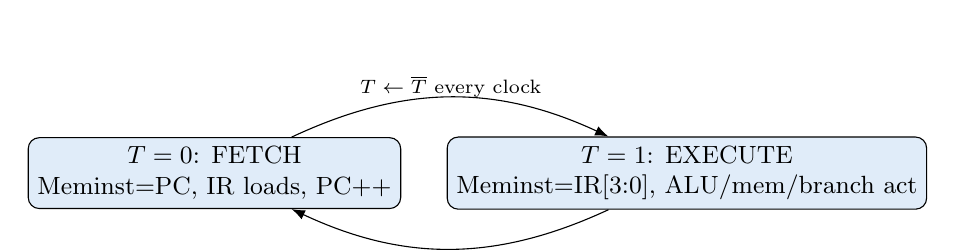
\begin{tikzpicture}[state/.style={draw, rounded corners, fill=boxblue, minimum width=3.4cm, minimum height=0.9cm, font=\small, align=center}, >=Latex]
\node[state] (t0) at (0,0)  {$T=0$: FETCH\\Meminst$=$PC, IR loads, PC${+}{+}$};
\node[state] (t1) at (6,0)  {$T=1$: EXECUTE\\Meminst$=$IR[3:0], ALU/mem/branch act};
\draw[->] (t0) to[bend left=25] (t1);
\draw[->] (t1) to[bend left=25] (t0);
\node at (3,1.1) {\scriptsize $T \leftarrow \overline{T}$ every clock};
\end{tikzpicture}
\caption{The only sequencing element: a single toggle flip-flop $T$
(Fetch/Execute phase), \emph{not} a multi-state FSM. Everything else in
\S\ref{sec:isa}'s control table is a pure function of the current opcode,
$T$, and the zero flag.}
\label{fig:phase}
\end{figure}

\subsection*{Component Summary}

\begin{center}
\begin{tabular}{@{}p{2.9cm}p{9.5cm}@{}}
\toprule
\textbf{Block} & \textbf{Purpose} \\
\midrule
PC (Program Counter) & 4-bit register; increments at the end of
\texttt{FETCH} ($T{=}0{\to}1$); loaded from \texttt{IR[3:0]} instead, at
the end of \texttt{EXECUTE}, when \texttt{PC\_load} is asserted (branch
taken). \\
Meminst mux & 2:1 multiplexer (not a register) selecting RAM's address:
\texttt{PC} when $T{=}0$, \texttt{IR[3:0]} when $T{=}1$. \\
RAM & 16 $\times$ 8-bit memory holding program and data. Address from the
Meminst mux; \texttt{Din}$=$ACC, \texttt{WE}$=$\texttt{MemWr} (write only
for \texttt{STA}, only at $T{=}1$). \\
IR (Instruction Register) & 8-bit register, loaded from RAM's data output
only during \texttt{FETCH} ($T{=}0$). Its opcode nibble feeds the
Hardwired Control Logic; its operand nibble feeds the Meminst mux and
PC's branch-load input. \\
ACC (Accumulator) & The only general-purpose data register. Feeds the
ALU's $A$ input, RAM's data-in port (for \texttt{STA}), and a 4-input NOR
``zero flag'' detector; loaded from the ACC-source mux. \\
ALU & Provided \texttt{ALU\_4} circuit (\S 2). $A{=}$ACC, $B{=}$RAM data
(tapped before IR), $S[2{:}0]$ from the Hardwired Control Logic. \\
Hardwired Control Logic & Purely combinational (no internal state):
reads \texttt{IR[7:4]}, $Z$ and $T$, and drives every load-enable, mux
select and $S[2{:}0]$ in the table below. \\
\bottomrule
\end{tabular}
\end{center}

\section{Instruction Set Architecture}
\label{sec:isa}

Each instruction occupies \textbf{one 8-bit memory word}: a 4-bit
\textbf{opcode} in the upper nibble and a 4-bit \textbf{operand} (a
memory address, doubling as a branch target) in the lower nibble.

\begin{longtable}{@{}clp{6.4cm}c@{}}
\toprule
\textbf{Opcode} & \textbf{Mnemonic} & \textbf{Operation} & \textbf{ALU $S$} \\
\midrule
\texttt{0000} & NOP        & No operation.                                            & --- \\
\texttt{0001} & LDA addr   & $ACC \leftarrow M[addr]$                                & --- \\
\texttt{0010} & STA addr   & $M[addr] \leftarrow ACC$                                & --- \\
\texttt{0011} & ADD addr   & $ACC \leftarrow ACC + M[addr]$                          & \texttt{000} \\
\texttt{0100} & SUB addr   & $ACC \leftarrow ACC - M[addr]$                          & \texttt{001} \\
\texttt{0101} & AND addr   & $ACC \leftarrow ACC \wedge M[addr]$                     & \texttt{010} \\
\texttt{0110} & OR addr    & $ACC \leftarrow ACC \vee M[addr]$                       & \texttt{011} \\
\texttt{0111} & JMP addr   & $PC \leftarrow addr$ (unconditional branch)             & --- \\
\texttt{1000} & JZ addr    & if $ACC = 0$: $PC \leftarrow addr$ (conditional branch) & --- \\
\texttt{1001} & HLT        & Halt: gate off the clock enable.                        & --- \\
\bottomrule
\caption{The 10-instruction ISA. Opcodes \texttt{1010}--\texttt{1111} are
unused and reserved.}
\end{longtable}

\subsection*{Hardwired Control Logic}

Two of the eight control signals need no decode logic at all -- they are
a direct (inverted, for one) wire from the phase flip-flop $T$:
$\mathtt{Meminst\_sel} = T$ and $\mathtt{IRload} = \overline{T}$. The
remaining six depend on the opcode $O_3O_2O_1O_0=$\,\texttt{IR[7:4]}
(and, for \texttt{PC\_load}, the zero flag $Z$), and are only meant to
act during \texttt{EXECUTE} ($T{=}1$):

\begin{center}
\begin{tabular}{@{}clccccc@{}}
\toprule
\textbf{Opcode} & \textbf{Mnemonic} & \textbf{ACC\_load} & \textbf{ACC\_src} & \textbf{MemWr} & \textbf{PC\_load} & \textbf{HLT} \\
\midrule
0000 & NOP & 0 & --- & 0 & 0 & 0 \\
0001 & LDA & 1 & RAM  & 0 & 0 & 0 \\
0010 & STA & 0 & ---  & 1 & 0 & 0 \\
0011 & ADD & 1 & ALU  & 0 & 0 & 0 \\
0100 & SUB & 1 & ALU  & 0 & 0 & 0 \\
0101 & AND & 1 & ALU  & 0 & 0 & 0 \\
0110 & OR  & 1 & ALU  & 0 & 0 & 0 \\
0111 & JMP & 0 & ---  & 0 & 1 & 0 \\
1000 & JZ  & 0 & ---  & 0 & $Z$ & 0 \\
1001 & HLT & 0 & ---  & 0 & 0 & 1 \\
\bottomrule
\end{tabular}
\end{center}

(all six columns are additionally ANDed with $T$, since they must stay
inactive during \texttt{FETCH}). \texttt{ACC\_src} selects \texttt{RAM}
data for \texttt{LDA} and the \texttt{ALU} result for the four
arithmetic/logic opcodes; $S[2{:}0]$ is \texttt{000/001/010/011} for
\texttt{ADD/SUB/AND/OR} respectively and don't-care otherwise. Every
column here is a small, fixed function of 4 (or 5) input bits -- buildable
directly as a two-level AND--OR circuit, or as a tiny lookup table -- with
\emph{no} states, and \emph{no} sequencing beyond the single phase bit
$T$. This is what it means for \textbf{the control signal to live in the
instruction itself}, decoded freshly every cycle, rather than in a
separate multi-state control unit.

\task{1.5 --- Derive it yourself.} Before wiring up the table above, pick
one column (e.g.\ \texttt{ACC\_load}) and derive its minimal AND--OR
expression directly from the ISA table yourself. Compare your gate count
against a classmate's.

\section{Build Tasks}

Work through the tasks in order. Test each block in isolation before
wiring it into the full CPU --- debugging a single register is far easier
than debugging the whole machine at once.

\task{2 --- Registers.} Build 4-bit \texttt{PC} and \texttt{ACC}, and an
8-bit \texttt{IR}, using Logisim's \textbf{Register} component, each with
a separate \emph{load enable} input. There is \textbf{no MAR} to build.
Add the 1-bit phase flip-flop $T$ (a D flip-flop wired as $T \leftarrow
\overline{T}$, i.e.\ toggling every clock edge).

\task{3 --- Memory and the Meminst mux.} Add a 16 $\times$ 8-bit
\textbf{RAM} component. Build the \textbf{Meminst} 2:1 multiplexer feeding
its address input directly from \texttt{PC} (when $T{=}0$) or
\texttt{IR[3:0]} (when $T{=}1$) -- this replaces the MAR entirely. Use the
\emph{Load Image} feature (right-click $\to$ ``Load Image'') to pre-load a
hex program image once you have written one (\S\ref{sec:testprog}).

\task{4 --- ALU and ACC-source mux.} Wire \texttt{ACC} to the ALU's $A$
input, and RAM's data output (tapped \emph{before} \texttt{IR}) to the
ALU's $B$ input, as point-to-point wires -- no bus. Build the ACC-source
mux (RAM data vs.\ ALU result $F$) feeding \texttt{ACC}'s data input, and
wire \texttt{ACC}'s output to RAM's data-in port for \texttt{STA}.

\task{5 --- Hardwired Control Logic.} Build the six opcode-decoded
signals from the truth table in \S\ref{sec:isa} (\texttt{ACC\_load},
\texttt{ACC\_src}, \texttt{MemWr}, \texttt{PC\_load}, $S[2{:}0]$,
\texttt{HLT}) as plain combinational logic (AND/OR/NOT gates, or a small
lookup table) reading \texttt{IR[7:4]} and the zero flag $Z$. Remember to
AND each of them with $T$ so they are inactive during \texttt{FETCH}.
This is \emph{not} a state machine -- there are no flip-flops in this
task at all.

\task{6 --- Assemble the CPU.} Wire Tasks 2--5 together following
Figure~\ref{fig:datapath}. Add a manual clock (or Logisim's clock
component) with single-step capability so you can observe \texttt{FETCH}
and \texttt{EXECUTE} separately on the Poke tool / Logisim's built-in
\emph{Hex Editor} and \emph{Log}.

\section{Test Program}
\label{sec:testprog}

Hand-assemble and run the following program, which computes $5 + 3$, stores
the result, then loops decrementing a counter down to zero using the
conditional branch. All 16 words of memory (addresses \texttt{0}--\texttt{F})
are used, with instructions in \texttt{0}--\texttt{8} and data/constants in
\texttt{B}--\texttt{F}: no address is shared between code and data.

\begin{lstlisting}
; addr : instruction   ; encoding (opcode|operand)   ; comment
0 : LDA E              ; 0001 1110                   ; ACC <- M[E] = 5
1 : ADD F              ; 0011 1111                   ; ACC <- ACC + M[F] = 5+3 = 8
2 : STA D              ; 0010 1101                   ; M[D] <- ACC   (result = 8)
3 : LDA C              ; 0001 1100                   ; ACC <- M[C]   (loop counter)
4 : SUB B              ; 0100 1011                   ; ACC <- ACC - M[B]  (counter - 1)
5 : STA C              ; 0010 1100                   ; M[C] <- ACC   (store new counter)
6 : JZ  8              ; 1000 1000                   ; if ACC = 0 goto HLT
7 : JMP 3              ; 0111 0011                   ; else repeat loop
8 : HLT                ; 1001 0000                   ; stop
9 : -                  ; 0000 0000                   ; unused
A : -                  ; 0000 0000                   ; unused
B : 1  (constant)      ; 0000 0001                   ; decrement amount
C : 3  (variable)      ; 0000 0011                   ; loop counter, initial value 3
D : 0  (variable)      ; 0000 0000                   ; result storage
E : 5  (constant)      ; 0000 0101                   ; first operand
F : 3  (constant)      ; 0000 0011                   ; second operand
\end{lstlisting}

\task{7 --- Verify.} Trace the program by hand first (fill in a
register-value table for PC/IR/ACC/M[C] on every clock tick), then run it
in Logisim and confirm your trace matches. \checkoff\ $M[D]$ ends at
\texttt{1000} (8). \checkoff\ $M[C]$ ends at \texttt{0000} (0) after three
passes through the loop. \checkoff\ The CPU halts (does not keep fetching
after \texttt{HLT}).

\task{8 --- Your own program.} Write and test a second program that uses
\texttt{AND}/\texttt{OR} and at least one branch, of your own design (e.g.
masking a value, or a 3-iteration loop that toggles a memory location).

\section{Deliverables}

\begin{itemize}[nosep]
  \item Your completed \texttt{.circ} file, containing the ALU (unmodified
        internals permitted to be re-wrapped as a subcircuit), registers,
        memory, the Meminst/ACC-source muxes, the Hardwired Control Logic,
        and the top-level CPU circuit.
  \item A short design note (1 page) showing the truth table or Boolean
        equations you actually built for the six opcode-decoded control
        signals.
  \item Hand-trace tables and machine-code listings for both test programs
        (\S\ref{sec:testprog} and Task 8).
\end{itemize}

\section{Marking Guide}

\begin{center}
\begin{tabular}{@{}p{10.4cm}c@{}}
\toprule
\textbf{Criterion} & \textbf{Marks} \\
\midrule
ALU correctly integrated and verified & 10 \\
Registers (PC, IR, ACC) and phase flip-flop $T$ correct, independently testable & 15 \\
Meminst mux and RAM correctly addressed (no MAR) & 10 \\
Hardwired Control Logic correctly implements the \S\ref{sec:isa} table & 30 \\
All 10 instructions function correctly & 20 \\
Test program (\S\ref{sec:testprog}) runs correctly & 10 \\
Student-authored program (Task 8) & 5 \\
\midrule
\textbf{Total} & \textbf{100} \\
\bottomrule
\end{tabular}
\end{center}

\section*{Extension (Optional, not marked)}
Extend the ISA with an \texttt{OUT} instruction driving a 7-segment display,
or widen the datapath to 8 bits. Consider what changes to the Hardwired
Control Logic and ALU are required if you add an \texttt{XOR} or
\texttt{NOT} function using the two still-unused ALU select codes.

\end{document}
